\documentclass[12pt,a4paper]{article}
\usepackage{a4wide}
\usepackage{tikz}
\usetikzlibrary{arrows,shapes}
\usepackage[portuguese]{babel}
\usepackage[utf8]{inputenc} 
\usepackage{setspace}
\usepackage{indentfirst}


\begin{document}
\begin{titlepage}
\onehalfspacing

\newcommand{\HRule}{\rule{\linewidth}{0.5mm}} % Defines a new command for the horizontal lines, change thickness here

\center % Center everything on the page
 
%----------------------------------------------------------------------------------------
%    HEADING SECTIONS
%----------------------------------------------------------------------------------------

\textsc{\LARGE Universidade do Minho}\\[1.5cm] % Name of your university/college
\textsc{\Large Licenciatura em Engenharia Informática}\\[0.5cm] % Major heading such as course name
\textsc{\large Laboratórios de Informática V}\\[0.5cm] % Minor heading such as course title
\textsc{3º Ano, 2º Semestre, Ano lectivo 2012/2013}\\[0.5cm]

%----------------------------------------------------------------------------------------
%    TITLE SECTION
%----------------------------------------------------------------------------------------

\HRule \\[0.4cm]
\textsc{\Large ArqueoDB}\\[0.4cm] % Title of your document
\textsc{ \large Análise de Requisitos}\\[0.4cm] % Title of your document
\HRule \\[1.5cm]
 
%----------------------------------------------------------------------------------------
%    AUTHOR SECTION
%----------------------------------------------------------------------------------------

\textsc{\large Autores:}\\
{André Santos nº60994 \\ Daniel Araújo nº61058 \\ Daniel Carvalho nº61008\\ Helena Alves nº61000 \\ Pedro Carneiro nº61085}\\[1cm] % Your name

%----------------------------------------------------------------------------------------
%    DATE SECTION
%----------------------------------------------------------------------------------------

Braga, {\large \today}\\[1cm] % Date, change the \today to a set date if you want to be precise

%----------------------------------------------------------------------------------------
%    LOGO SECTION
%----------------------------------------------------------------------------------------


\includegraphics[scale=1]{escola_eng.png}\\[0cm] % Include a department/university logo - this will require the graphicx package
 
%----------------------------------------------------------------------------------------

\vfill % Fill the rest of the page with whitespace

\end{titlepage}
\thispagestyle{empty}
\newpage

\section{Introdução}


\newpage

\section{Modelo de Domínio}
O modelo de domínio é um esquema que captura todas as entidades do sistema e todos os relacionamentos entre estas. Neste trabalho, foi desenvolvido um sistema de partilha de conhecimento sobre locais, achados e factos arqueológicos. A plataforma destinar-se-á, por um lado, aos profissionais e especialistas da área Arqueológica que, sobre a alçada de uma organização bem identificada, serão responsáveis por toda a gestão de informação relativa aos locais, achados ou factos mencionados e, por outro lado, ao utilizador regular com interesse na área que poderá ter acesso a toda essa informaçãoo de forma bastante interactiva. Desta forma, podem ser encontrados 4 tipos de utilizador: o utilizador visitante, o utilizador normal, o responsável e o profissional de uma dada organização. Sendo que o administrador é a entidade que gere a grande parte da informação do sistema:\\
\begin{itemize}
\item É o responável pelo controlo dos registos dos clientes no sistema;
\item É ele que administra, juntamente com os responsáveis de uma organização, todos os assuntos relacionados com a mesma;
\item É o responsável por gerir grande parte das utilidades do sistema.
\end{itemize}

Na página seginte á apresentado o modelo de domínio correspondente ao nosso sistema.
\newpage

\begin{figure}[h!]
\centering
\includegraphics[scale=1]{}
\label{modelo domínio}
\caption{Modelo de Domínio}
\end{figure}


\newpage
\section{Diagrama de Use Cases}
Um diagrama de use cases é um diagrama onde são representados todos os actores envolventes de um dado sistema, assim como todas as acções que estes podem executar. Devido à incapacidade de colocar o diagrama de use cases, numa só página, devido ao seu tamanho, este foi dividido em três partes. Desta forma, este é apresentado de seguida:\\

\begin{figure}[h!]
\centering
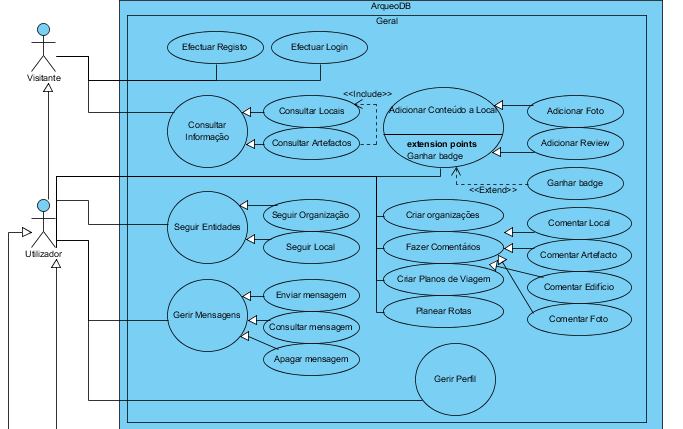
\includegraphics[scale=1]{usecase/geral1}
\label{usecase}
\caption{Diagrama de Use Cases}
\end{figure}

\begin{figure}[h!]
\centering
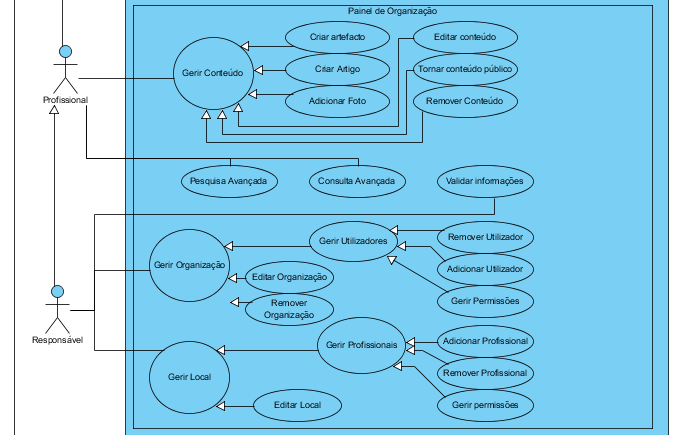
\includegraphics[scale=1]{usecase/geral2}
\label{usecase}
\caption{Diagrama de Use Cases}
\end{figure}

\begin{figure}[h!]
\centering
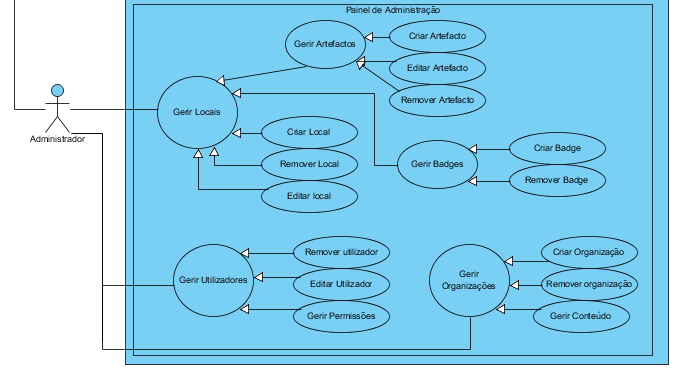
\includegraphics[scale=1]{usecase/geral3}
\label{usecase}
\caption{Diagrama de Use Cases}
\end{figure}

\clearpage

Neste diagrama estão representados todos os sub-sistemas do sistema ArqueoDB, incluindo todos os actores e suas acções. Para promover uma  melhor compreensão, vão ser apresentados cada um destes sub-sistemas individualmente, juntamente com as especificações textuais de cada use case corresponde ao respecivo sub-sistema. \\


\subsection{Sub-sistema Acesso ao sistema}
Neste subsistema é possível os utilizadores efectuarem o seu registo no sistema. Contudo, tanto utilizadores como administrador podem efectuar o login no sistema, quando necessitarem de entrar no sitema.\\

\begin{figure}[h!]
\centering
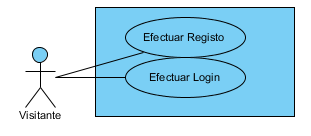
\includegraphics[scale=1]{usecase/U_AcessoSistema}
\label{usecase}
\caption{Diagrama de Use Cases do sub-sistema Acesso ao sistema}
\end{figure}

De seguida, encontram-se as especificações textuais dos use cases do diagrama deste sub-sistema:\\

\begin{figure}[h!]
\centering
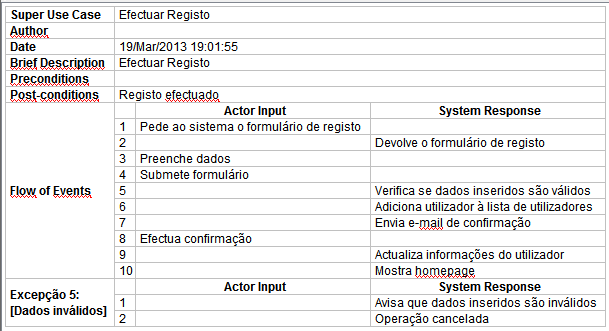
\includegraphics[scale=0.7]{d_usecase/registo}
\label{usecase}
\caption{Detalhes use case efectuar registo}
\end{figure}

\clearpage
\newpage

\begin{figure}[h!]
\centering
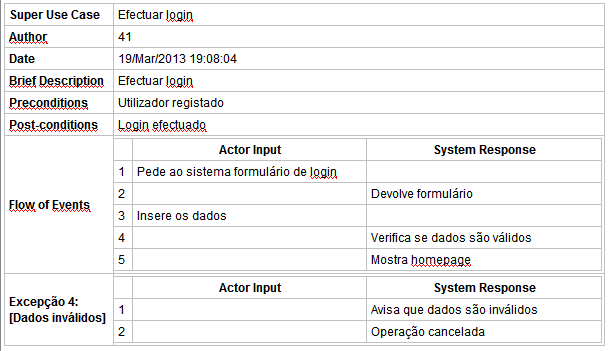
\includegraphics[scale=0.7]{d_usecase/login}
\label{usecase}
\caption{Detalhes use case efectuar login}
\end{figure}

\subsection{Sub-sistema Consultar Informação}
Neste sub-sistema está representado o utilizador ``visitante'', além de que, como pode ser verificado no diagrama de use case geral, todos os outros tipos de utilizador podem executar todas as acções realizadas por este. Deste modo, os utilizadores têm como actividade, representada neste diagrama, a consulta de informação, nomeadamente, a consulta de locais e artefactos.\\

\begin{figure}[h!]
\centering
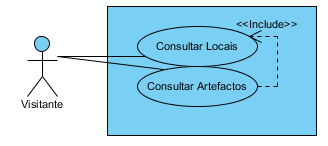
\includegraphics[scale=1]{usecase/V_ConsultarInformaccao}
\label{usecase}
\caption{Diagrama de Use Cases do sub-sistema Consultar Informação}
\end{figure}

De seguida, encontram-se as especificações textuais dos use cases do diagrama deste sub-sistema:\\


\begin{figure}[h!]
\centering
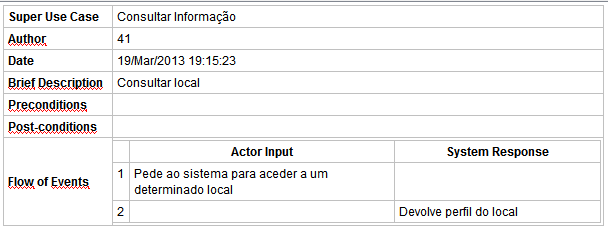
\includegraphics[scale=0.7]{d_usecase/consultarlocais}
\label{usecase}
\caption{Detalhes use case consultar local}
\end{figure}


\begin{figure}[h!]
\centering
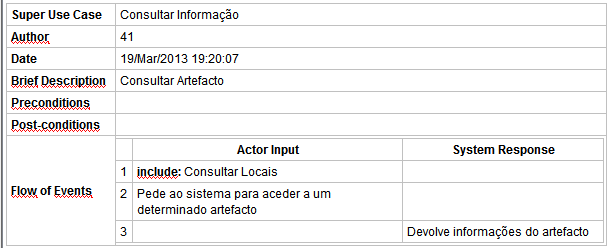
\includegraphics[scale=0.7]{d_usecase/consultarartefacto}
\label{usecase}
\caption{Detalhes use case consultar artefacto}
\end{figure}

\subsection{Sub-sistema Seguir entidades}
No diagrama use case deste sub-sistema estão envolvidas as duas possibilidades que o utilizador pode tomar, em relação a seguir entidades. Pode, no entanto, seguir determinado local ou determinada organização. Estas acções podem ser executados pelo utilizador, o profissional e o responsável de uma organização.\\

\begin{figure}[h!]
\centering
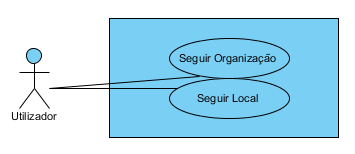
\includegraphics[scale=1]{usecase/U_SeguirEntidades}
\label{usecase}
\caption{Diagrama de Use Cases do sub-sistema Seguir Entidades}
\end{figure}

De seguida, encontram-se as especificações textuais dos use cases do diagrama deste sub-sistema:\\


\begin{figure}[h!]
\centering
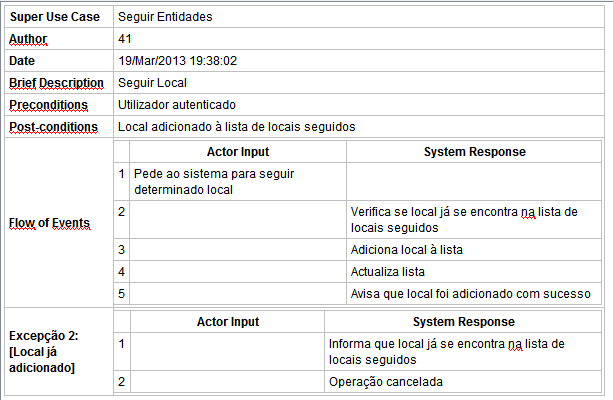
\includegraphics[scale=0.7]{d_usecase/seguirlocal}
\label{usecase}
\caption{Detalhes use case seguir local}
\end{figure}

\begin{figure}[h!]
\centering
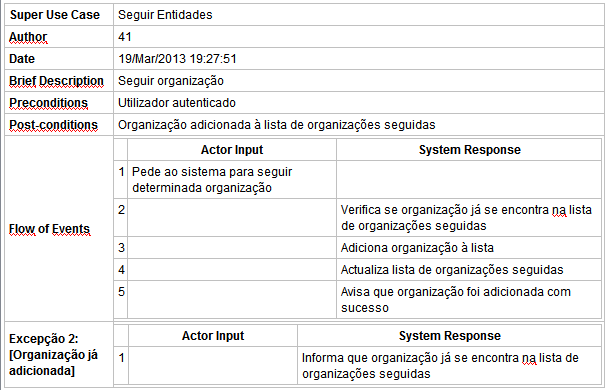
\includegraphics[scale=0.7]{d_usecase/seguirorganizacao}
\label{usecase}
\caption{Detalhes use case seguir organizacao}
\end{figure}

\newpage
\subsection{Sub-sistema Gerir perfil do utilizadoor}
Este sub-sistema permite ao utilizador, a qualquer momento, alterar as suas definições pessoais.\\

\begin{figure}[h!]
\centering
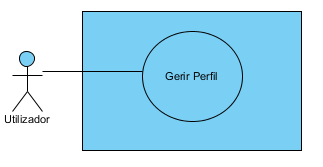
\includegraphics[scale=1]{usecase/U_GerirPerfil}
\label{usecase}
\caption{Diagrama Use Case sub-sistema Gerir Perfil}
\end{figure}

De seguida, encontra-se a especificação textual do único use case do diagrama deste sub-sistema:\\

\begin{figure}[h!]
\centering
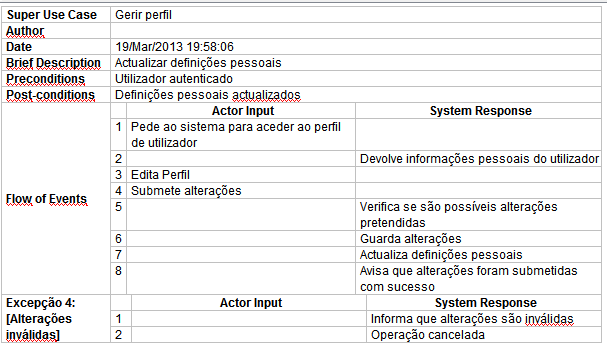
\includegraphics[scale=0.7]{d_usecase/gerirperfil}
\label{usecase}
\caption{Detalhes use case Gerir Perfil}
\end{figure}

\newpage
\subsection{Sub-sistema Gestão de mensagens do utilizador}
No diagrama de use case deste sub-sistema estão representadas todas as acções relativas à gestão de mensagens. É permitido aos vários tipos de utilizadores, registados no sistema, escrever, apagar mensagens e consultar a sua respectiva caixa de mensagens.\\

\begin{figure}[h!]
\centering
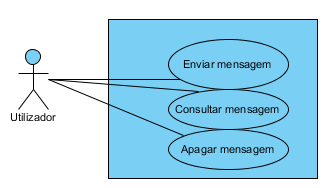
\includegraphics[scale=1]{usecase/U_GerirMensagens}
\label{usecase}
\caption{Diagrama Use Case sub-sistema Gerir mensagens}
\end{figure}

De seguida, encontram-se as especificações textuais dos use cases do diagrama deste sub-sistema:\\

\begin{figure}[h!]
\centering
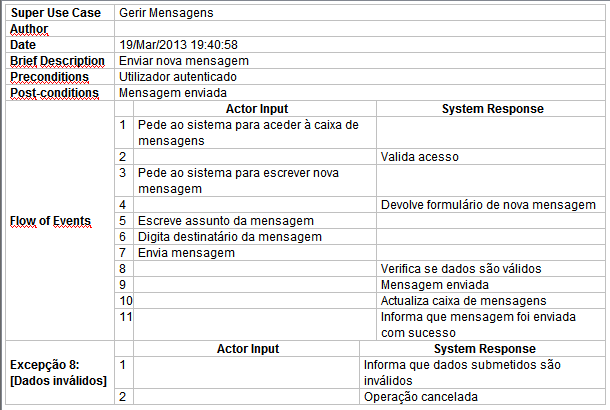
\includegraphics[scale=0.7]{d_usecase/enviarmensagem}
\label{usecase}
\caption{Detalhes use case Enviar nova mensagem}
\end{figure}

\begin{figure}[h!]
\centering
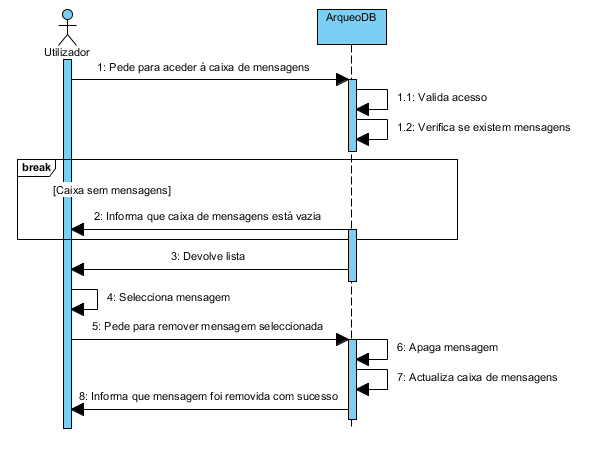
\includegraphics[scale=0.7]{d_usecase/apagarmensagem}
\label{usecase}
\caption{Detalhes use case Apagar mensagem}
\end{figure}

\begin{figure}[h!]
\centering
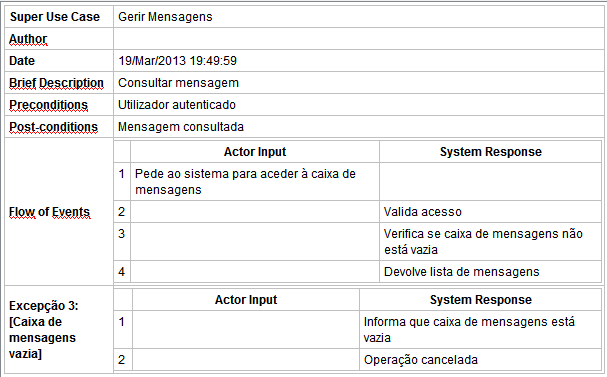
\includegraphics[scale=0.7]{d_usecase/consultarmensagem}
\label{usecase}
\caption{Detalhes use case Consultar mensagens}
\end{figure}

\clearpage
\newpage

\subsection{Sub-sistema Gestão de outras funcionalidades}
No diagrama de use case deste sub-sistema estão representadas todas outras funcionalidades acessíveis aos utilizadores. Estas dizem respeito à possibilidade de o utilizador criar planos de viagem, planear rotas e criar organizações. Estas funcionalidades exigem por parte do sistema uma verificação da possibilidade da concretização das mesmas, em que, caso não seja possível, o sistema devolve uma mensagem de erro, informando que a operação não pode ser realizada.\\

\begin{figure}[h!]
\centering
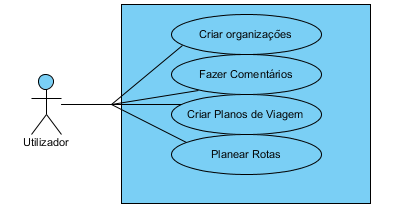
\includegraphics[scale=1]{usecase/U_FazerCenas}
\label{usecase}
\caption{Diagrama Use Case sub-sistema Gestão de outras funcionalidades}
\end{figure}

De seguida, encontram-se as especificações textuais dos use cases do diagrama deste sub-sistema:\\

\begin{figure}[h!]
\centering
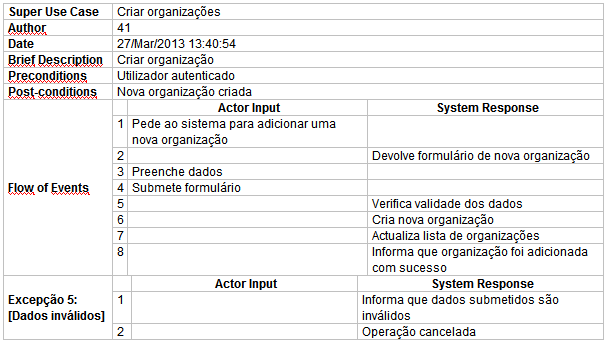
\includegraphics[scale=0.7]{d_usecase/criarorganizacao}
\label{usecase}
\caption{Detalhes use case Criar Organização}
\end{figure}

\begin{figure}[h!]
\centering
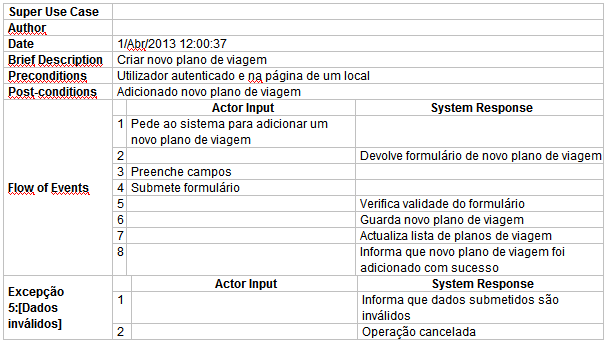
\includegraphics[scale=0.7]{d_usecase/criarviagem}
\label{usecase}
\caption{Detalhes use case Criar plano de viagem}
\end{figure}

\begin{figure}[h!]
\centering
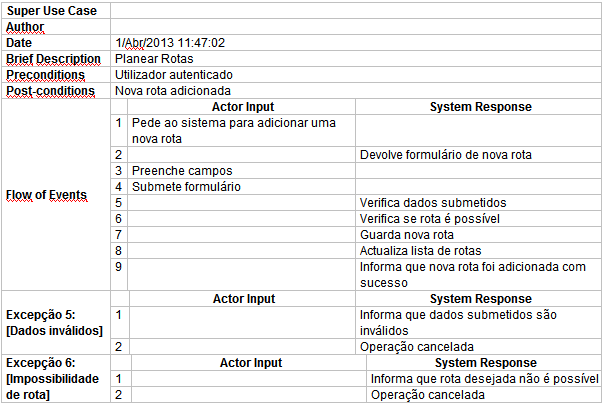
\includegraphics[scale=0.7]{d_usecase/planearrota}
\label{usecase}
\caption{Detalhes use case Planear Rotas}
\end{figure}

\clearpage
\newpage

\subsection{Sub-sistema Gestão de Comentários}
É neste sub-sistema que os utilizadores podem comentar determinado conteúdo. Sendo assim possível, um utilizador comentar um determinado local, um artefacto, um edifício ou uma foto. Para tal, basta o utilizador encontrar-se na página correspondente ao conteúdo que pretende comentar. Esta possibilidade de comentar determinado conteúdo é proporcionada a qualquer utilizador registado no sistema..  \\

\begin{figure}[h!]
\centering
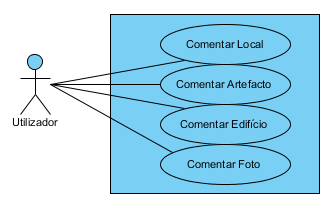
\includegraphics[scale=1]{usecase/U_FazerComentarios}
\label{usecase}
\caption{Diagrama Use Case sub-sistema Gestão de Comentários}
\end{figure}

De seguida, encontram-se as especificações textuais dos use cases do diagrama deste sub-sistema:\\

\begin{figure}[h!]
\centering
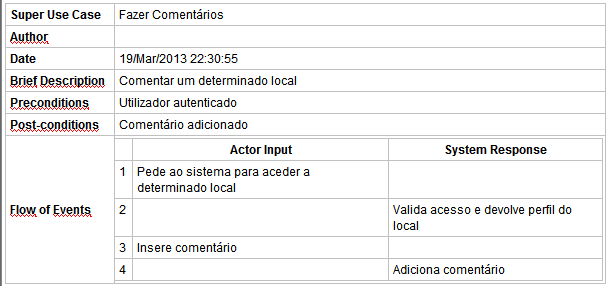
\includegraphics[scale=0.7]{d_usecase/comentarlocal}
\label{usecase}
\caption{Detalhes use case Comentar um local}
\end{figure}

\begin{figure}[h!]
\centering
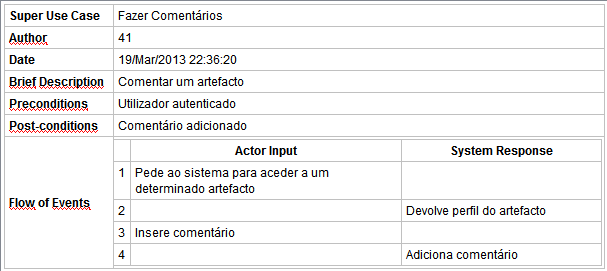
\includegraphics[scale=0.7]{d_usecase/comentarartefacto}
\label{usecase}
\caption{Detalhes use case Comentar Artefacto}
\end{figure}

\begin{figure}[h!]
\centering
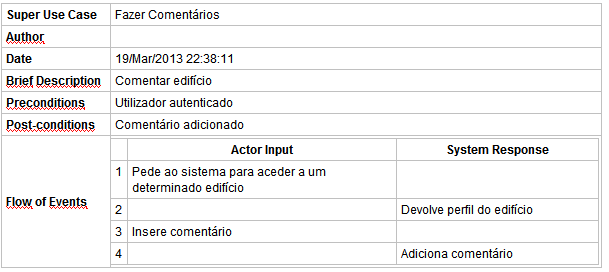
\includegraphics[scale=0.7]{d_usecase/comentaredificio}
\label{usecase}
\caption{Detalhes use case Comentar edifício}
\end{figure}

\begin{figure}[h!]
\centering
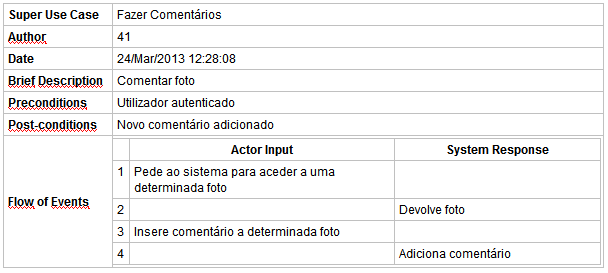
\includegraphics[scale=0.7]{d_usecase/comentarfoto}
\label{usecase}
\caption{Detalhes use case Comentar foto}
\end{figure}

\clearpage


\subsection{Sub-sistema Gestão de conteúdo}
No diagrama use case deste sub-sistema estão representadas acções relativas à gestão dos diversos conteúdos de uma determinada organização, podendo o responsável, como também o profissional da organização, criar artefactos, artigos, adicionar fotos, editar e remover conteúdo, como também torná-lo público.\\

\begin{figure}[h!]
\centering
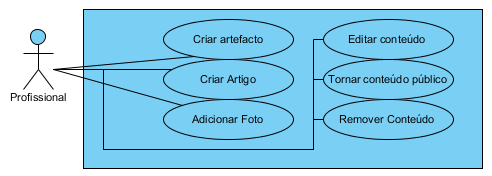
\includegraphics[scale=1]{usecase/P_GerirConteudo}
\label{usecase}
\caption{Diagrama Use Case sub-sistema Gestão de Conteúdo de uma organização}
\end{figure}

De seguida, encontram-se as especificações textuais dos use cases do diagrama deste sub-sistema:\\

\begin{figure}[h!]
\centering
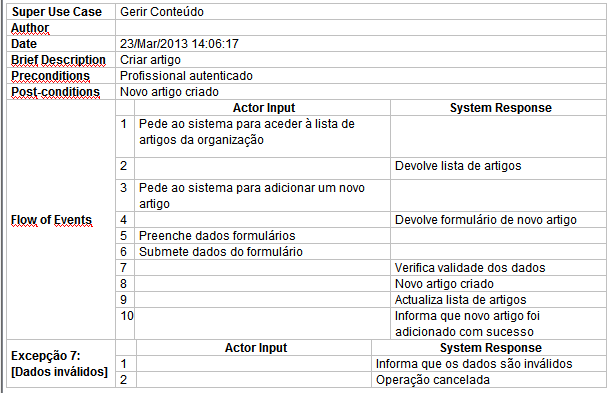
\includegraphics[scale=0.7]{d_usecase/criarartigo}
\label{usecase}
\caption{Detalhes use case Criar artigo}
\end{figure}

\begin{figure}[h!]
\centering
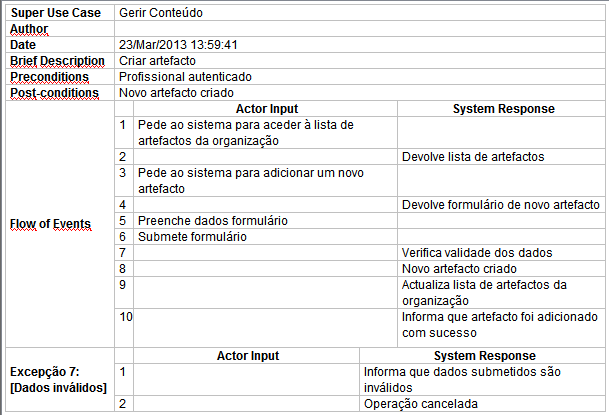
\includegraphics[scale=0.7]{d_usecase/criarartefacto}
\label{usecase}
\caption{Detalhes use case Criar artefacto}
\end{figure}

\begin{figure}[h!]
\centering
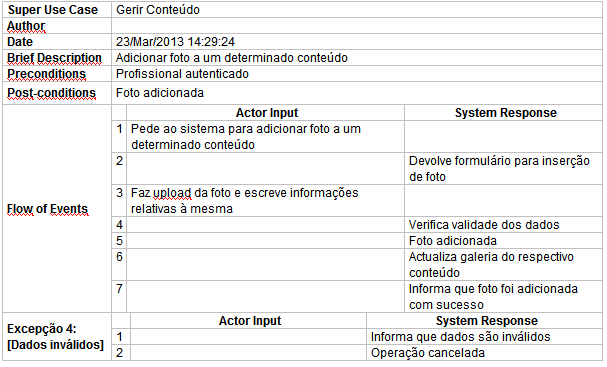
\includegraphics[scale=0.7]{d_usecase/P_adicionarfoto}
\label{usecase}
\caption{Detalhes use case Adicionar foto a determinado conteúdo}
\end{figure}

\begin{figure}[h!]
\centering
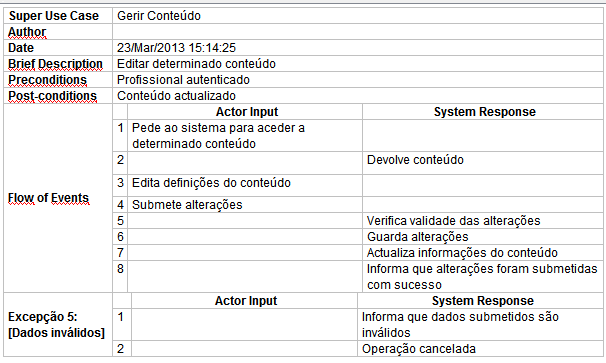
\includegraphics[scale=0.7]{d_usecase/editarconteudo}
\label{usecase}
\caption{Detalhes use case Editar conteúdo de uma organização}
\end{figure}

\begin{figure}[h!]
\centering
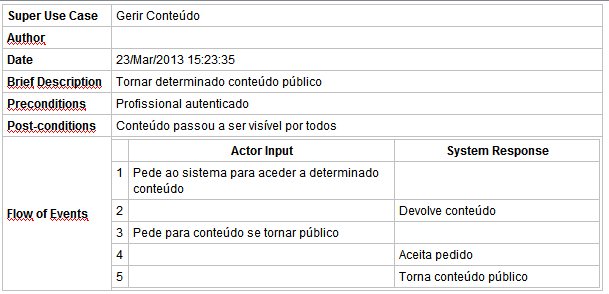
\includegraphics[scale=0.7]{d_usecase/tornarpublico}
\label{usecase}
\caption{Detalhes use case Tornar público determinado conteúdo}
\end{figure}

\begin{figure}[h!]
\centering
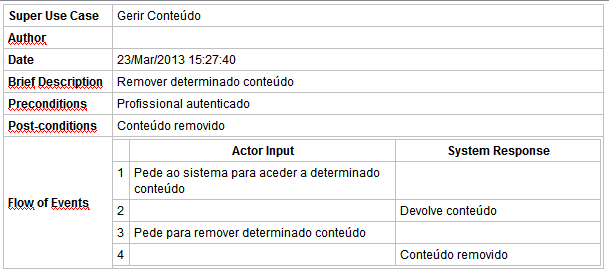
\includegraphics[scale=0.7]{d_usecase/removerconteudo}
\label{usecase}
\caption{Detalhes use case Remover conteúdo de uma organização}
\end{figure}


\clearpage
\clearpage
\subsection{Sub-sistema Gestão da organização}
No diagrama use case deste sub-sistema estão representadas acções relativas à gestão de uma dada organização a que o utilizador pertença, sendo estas acções apenas relativas ao responsável pela organização. O responsável pode editar as definições da organização, remover a organização, assim como também gerir os utilizadores que fazem parte da mesma.\\

\begin{figure}[h!]
\centering
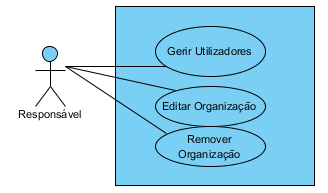
\includegraphics[scale=1]{usecase/R_GerirOrganizacao}
\label{usecase}
\caption{Diagrama Use Case sub-sistema Gestão da organização}
\end{figure}

De seguida, encontram-se as especificações textuais dos use cases do diagrama deste sub-sistema:\\

\begin{figure}[h!]
\centering
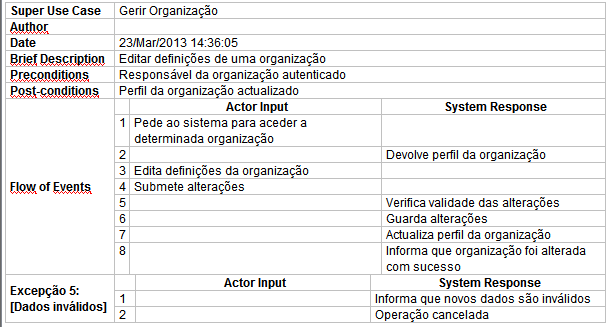
\includegraphics[scale=0.7]{d_usecase/editarorganizacao}
\label{usecase}
\caption{Detalhes use case Editar Organização}
\end{figure}

\begin{figure}[h!]
\centering
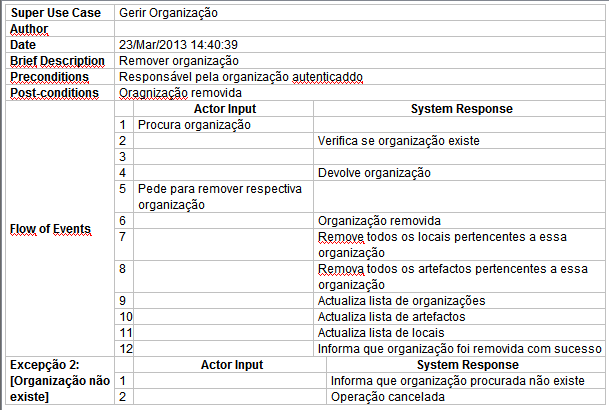
\includegraphics[scale=0.7]{d_usecase/removerorganizacao}
\label{usecase}
\caption{Detalhes use case Remover Organização}
\end{figure}

\clearpage

\subsection{Sub-sistema Gestão dos Utilizadores de uma organização}
No diagrama use case deste sistema estão representadas acções relativas apenas ao responsável de uma organização. Estas acções permitem ao responsável gerir os utilizadores pertencentes à sua organização, podendo adicionar e remover utilizadores, e também gerir as permissões dos mesmos, decidindo o que estes podem ou não fazer.\\

\begin{figure}[h!]
\centering
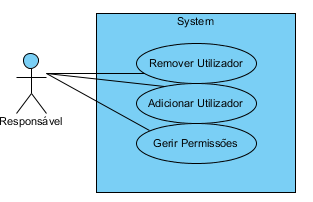
\includegraphics[scale=1]{usecase/R_GerirUtilizadores}
\label{usecase}
\caption{Diagrama Use Case sub-sistema Gestão da organização}
\end{figure}

De seguida, encontram-se as especificações textuais dos use cases do diagrama deste sub-sistema:\\

\begin{figure}[h!]
\centering
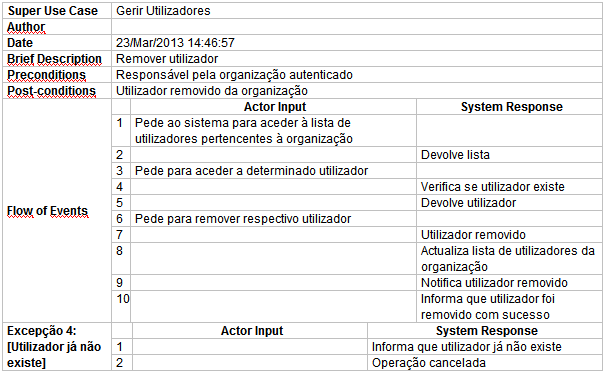
\includegraphics[scale=0.7]{d_usecase/removerutilizador}
\label{usecase}
\caption{Detalhes use case Remover utilizador de uma organização}
\end{figure}

\begin{figure}[h!]
\centering
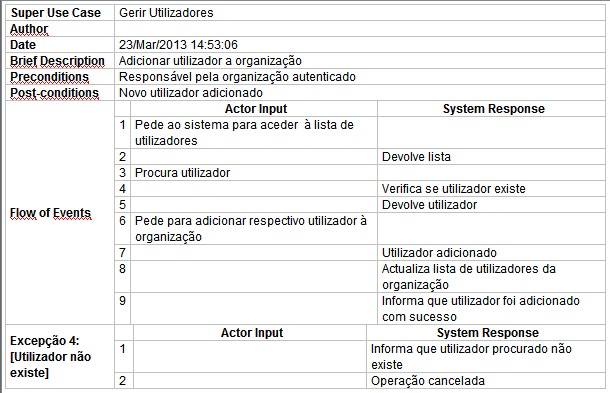
\includegraphics[scale=0.7]{d_usecase/adicionarutilizador}
\label{usecase}
\caption{Detalhes use case Adicionar utilizador a uma organização}
\end{figure}

\begin{figure}[h!]
\centering
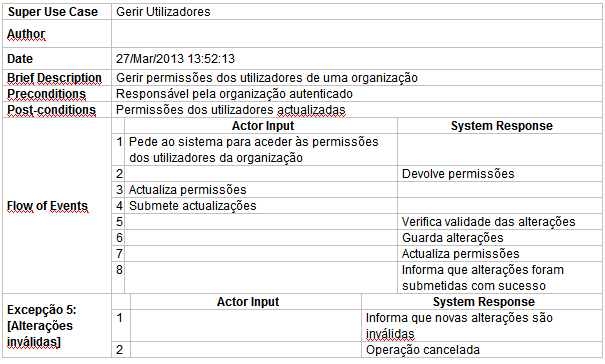
\includegraphics[scale=0.7]{d_usecase/R_permissoes}
\label{usecase}
\caption{Detalhes use case Gerir permissões dos utilizadores de uma organização}
\end{figure}

\clearpage
\clearpage

\subsection{Sub-sistema Gestão dos Locais de uma organização}
No diagrama use case deste sistema estão representadas, mais uma vez, acções relativas
apenas ao responsável ao responsável de uma organização. Estas acções permitema ao responsável gerir todos os locais pertencentes à sua organização, como alterar as definições do local, como também gerir os profissionais responsáveis pelo respectivo local.\\

\begin{figure}[h!]
\centering
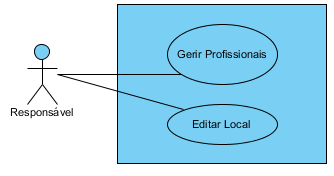
\includegraphics[scale=1]{usecase/R_GerirLocal}
\label{usecase}
\caption{Diagrama Use Case sub-sistema Gestão de Locais}
\end{figure}

De seguida, encontram-se as especificações textuais dos use cases do diagrama deste sub-sistema:\\

\begin{figure}[h!]
\centering
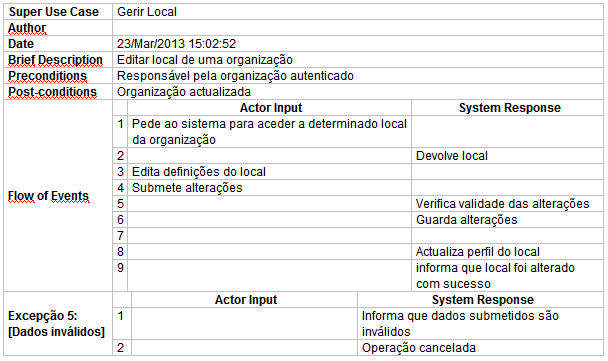
\includegraphics[scale=0.7]{d_usecase/editarlocal}
\label{usecase}
\caption{Detalhes use case Editar local}
\end{figure}

\subsection{Sub-sistema Gestão de profissionais de uma organização}
Este sub-sistema apenas envolve um actor, nomeadamente o responsável por uma organização. O diagrama
use case deste subsistema é relativo à gestão dos profissionais de uma organização, onde o responsável pela mesma pode adicionar novos utilizadores, remover utilizadores já pertencentes à organização, e também gerir ar permissões de todos os profissionais.\\

\begin{figure}[h!]
\centering
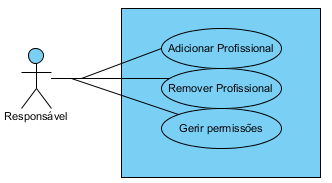
\includegraphics[scale=1]{usecase/R_GerirProfissionais}
\label{usecase}
\caption{Diagrama Use Case sub-sistema Gestão dos Profissionais de uma Organização}
\end{figure}

De seguida, encontram-se as especificações textuais dos use cases do diagrama deste sub-sistema:\\

\begin{figure}[h!]
\centering
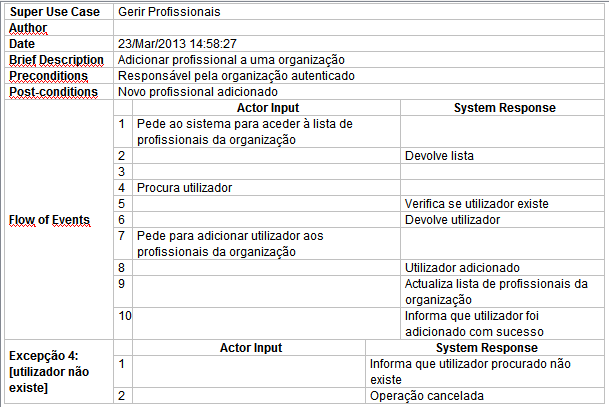
\includegraphics[scale=0.7]{d_usecase/adicionarprofissional}
\label{usecase}
\caption{Detalhes use case Adicionar profissional à organização}
\end{figure}



\begin{figure}[h!]
\centering
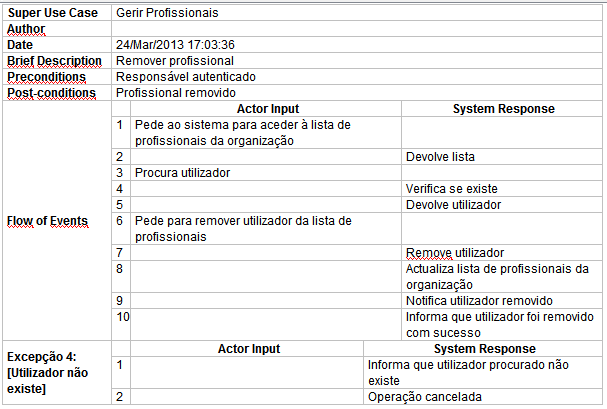
\includegraphics[scale=0.7]{d_usecase/removerprofissional}
\label{usecase}
\caption{Detalhes use case Remover profissional de uma organização}
\end{figure}

\begin{figure}[h!]
\centering
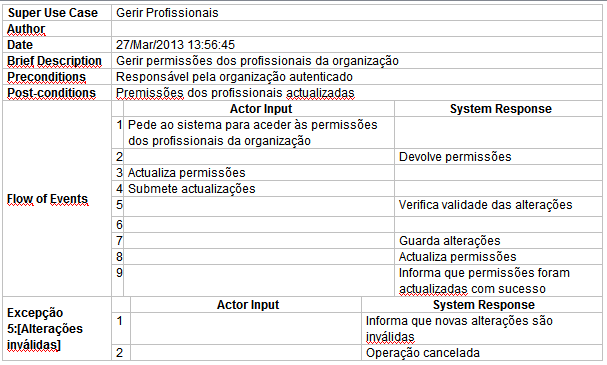
\includegraphics[scale=0.7]{d_usecase/P_permissoes}
\label{usecase}
\caption{Detalhes use case Gerir permissões dos profissionais de uma organização}
\end{figure}

\clearpage

\subsection{Sub-sistema Gestão de Locais do Sistema}
No diagrama use case deste sub-sistema estão representadas acções como adicionar, editar e remover locais de todo o sistema. Estas acções dizem respeito à gestão de locais, que só podem ser efectuadas pelo administrador. Ainda neste use case, é permitido ao utilizador gerir os artefactos e as badges pertencentes ao respectivo local.\\

\begin{figure}[h!]
\centering
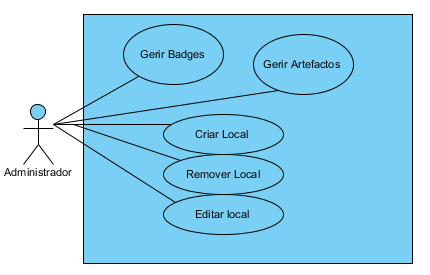
\includegraphics[scale=1]{usecase/A_GerirLocal}
\label{usecase}
\caption{Diagrama Use Case sub-sistema Gestão dos Locais do Sistema}
\end{figure}

De seguida, encontram-se as especificações textuais dos use cases do diagrama deste sub-sistema:\\

\begin{figure}[h!]
\centering
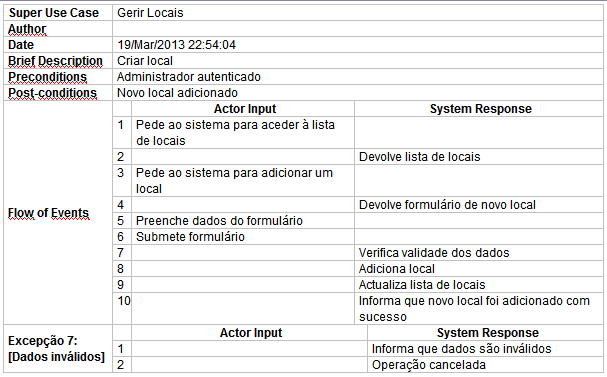
\includegraphics[scale=0.7]{d_usecase/A_criarlocal}
\label{usecase}
\caption{Detalhes use case Adicionar novo local ao sistema}
\end{figure}

\begin{figure}[h!]
\centering
\includegraphics[scale=0.7]{d_usecase/A_removerlocal}
\label{usecase}
\caption{Detalhes use case Remover local do sistema}
\end{figure}

\begin{figure}[h!]
\centering
\includegraphics[scale=0.7]{d_usecase/A_editarlocal}
\label{usecase}
\caption{Detalhes use case Editar um local}
\end{figure}

\clearpage

\subsection{Sub-sistema Gestão de Artefactos do Sistema}

O diagrama use case deste sub-sistema apresenta mais acções que o administrador do sistema
pode tomar. Estas acções estão relacionadas com a gestão dos artefactos do sistema. Aqui, o
administrador pode criar novos atefactos, modificar e remover artefactos já existentes.\\

\begin{figure}[h!]
\centering
\includegraphics[scale=1]{usecase/A_GerirLocal}
\label{usecase}
\caption{Diagrama Use Case sub-sistema Gestão dos Locais do Sistema}
\end{figure}

De seguida, encontram-se as especificações textuais dos use cases do diagrama deste sub-sistema:\\

\begin{figure}[h!]
\centering
\includegraphics[scale=0.7]{d_usecase/A_criarartefacto}
\label{usecase}
\caption{Detalhes use case Adicionar novo artefacto ao sistema}
\end{figure}

\begin{figure}[h!]
\centering
\includegraphics[scale=0.7]{d_usecase/A_removerartefacto}
\label{usecase}
\caption{Detalhes use case Remover artefacto do sistema}
\end{figure}

\begin{figure}[h!]
\centering
\includegraphics[scale=0.7]{d_usecase/A_editarartefacto}
\label{usecase}
\caption{Detalhes use case Editar um artefacto}
\end{figure}

\clearpage

\subsection{Sub-sistema Gestão de badges}
É neste sub-sistema que os administradores podem controlar as badges do sistema. O
adiministrador pode ser capaz de criar novas restriçõe, como também removê-las.\\

\begin{figure}[h!]
\centering
\includegraphics[scale=1]{usecase/A_GerirBadges}
\label{usecase}
\caption{Diagrama Use Case sub-sistema Gestão das Badges do Sistema}
\end{figure}

De seguida, encontram-se as especificações textuais dos use cases do diagrama deste sub-sistema:\\

\begin{figure}[h!]
\centering
\includegraphics[scale=0.7]{d_usecase/A_criarbadge}
\label{usecase}
\caption{Detalhes use case Adicionar nova badge ao sistema}
\end{figure}

\begin{figure}[h!]
\centering
\includegraphics[scale=0.7]{d_usecase/A_removerbadge}
\label{usecase}
\caption{Detalhes use case Remover badge do sistema}
\end{figure}

\clearpage

\subsection{Sub-sistema Gestão dos Utilizadores do Sistema}
No diagrama de use case deste sub-sistema estão representadas todas as acções relativas
à gestão dos utilizadores do sistema. É permitido ao administrador remover um utilizador, editar as definições do mesmo, como também gerir as permissões de todos os utilizadores do sistema. \\

\begin{figure}[h!]
\centering
\includegraphics[scale=1]{usecase/A_GerirUtilizadores}
\label{usecase}
\caption{Diagrama Use Case sub-sistema Gestão dos Utilizadores do Sistema}
\end{figure}

De seguida, encontram-se as especificações textuais dos use cases do diagrama deste sub-sistema:\\

\begin{figure}[h!]
\centering
\includegraphics[scale=0.7]{d_usecase/A_editarutilizador}
\label{usecase}
\caption{Detalhes use case Editar utilizador do sistema}
\end{figure}

\begin{figure}[h!]
\centering
\includegraphics[scale=0.7]{d_usecase/A_removerutilizador}
\label{usecase}
\caption{Detalhes use case Remover utilizador do sistema}
\end{figure}

\begin{figure}[h!]
\centering
\includegraphics[scale=0.7]{d_usecase/A_permissoes}
\label{usecase}
\caption{Detalhes use case Gerir permissões dos utilizadores do sistema} 
\end{figure}

\clearpage

\subsection{Sub-sistema Gestão das Organizações do Sistema}
O diagrama use case deste sistema apresenta mais acções que o administrador do sistema
pode tomar. Estas acções estão relacionadas com a gestão das organizações do sistema. Aqui, o
administardor pode criar novas organiuzações, remover organizações já existentes e modificar qualquer organização do sistema. Neste sub-sistema, o administrador ainda pode gerir todo o conteúdo pertencente a uma organização.\\

\begin{figure}[h!]
\centering
\includegraphics[scale=1]{usecase/A_GerirOrganizacoes}
\label{usecase}
\caption{Diagrama Use Case sub-sistema Gestão das Organizações do Sistema}
\end{figure}

De seguida, encontram-se as especificações textuais dos use cases do diagrama deste sub-sistema:\\

\begin{figure}[h!]
\centering
\includegraphics[scale=0.7]{d_usecase/A_criarorganizacao}
\label{usecase}
\caption{Detalhes use case Criar nova organização no sistema}
\end{figure}

\begin{figure}[h!]
\centering
\includegraphics[scale=0.7]{d_usecase/A_removerorganizacao}
\label{usecase}
\caption{Detalhes use case Remover organização do sistema}
\end{figure}

\begin{figure}[h!]
\centering
\includegraphics[scale=0.7]{d_usecase/A_gerirconteudo}
\label{usecase}
\caption{Detalhes use case Gerir conteúdo das organizações do sistema} 
\end{figure}


\clearpage
\section{Diagramas de Sequência}
A utilização de diagramas de sequência permite representar a sequência de interacções, ou
seja, as mensagens passadas entre objectos, num determinado sistema. É descrito o comportamento
ao longo do tempo de um único caso de uso, onde é dada ênfase à ordenação temporal dos pedidos e respostas desenvolvidas nas interacções dos objectos num dado cenário. Também foram definidos diagramas de sequência com sub-sistemas.

Tendo sito em conta, os diagramas seguintes fazem referência às funcionalidades de efectuar registo e login no sistema, respectivamente.\\

\begin{figure}[h!]
\centering
\includegraphics[scale=1]{sequencia/login}
\caption{Diagrama de Sequência de Efectuar login no sistema} 
\end{figure}

\begin{figure}[h!]
\centering
\includegraphics[scale=1]{sequencia/registo}
\caption{Diagrama de Sequência de Efectuar regsito no sistema} 
\end{figure}

\clearpage

Os diagramas seguintes descrevem o processo de consultar determinada informação, como consultar locais e artefactos.\\

\begin{figure}[h!]
\centering
\includegraphics[scale=1]{sequencia/consultarlocais}
\caption{Diagrama de Sequência Consultar Locais} 
\end{figure}

\begin{figure}[h!]
\centering
\includegraphics[scale=1]{sequencia/consultarartefacto}
\caption{Diagrama de Sequência de Consultar Artefacto} 
\end{figure}

O diagrama anterior faz referência ao diagrama de consultar locais, uma vez que para consultar um artefacto, é  necessariamente preciso o utilizador encontrar-se na página do local.

\clearpage
Os diagramas seguintes referem-se à possibilidade de o utilizador poder adicionar conteúdo a um local, nomeadamente, adicionar uma foto ou adicionar uma review.\\

\begin{figure}[h!]
\centering
\includegraphics[scale=1]{sequencia/adicionarfoto}
\caption{Diagrama de Sequência Adicioanr foto a um local} 
\end{figure}

\begin{figure}[h!]
\centering
\includegraphics[scale=1]{sequencia/adicionarreview}
\caption{Diagrama de Sequência Adicionar review a um local} 
\end{figure}

\clearpage
Os diagramas seguintes referem-se à funcionalidade de começar a seguir uma organização ou um local.\\

\begin{figure}[h!]
\centering
\includegraphics[scale=0.8]{sequencia/seguirorganizacao}
\caption{Diagrama de Sequência Seguir Organização} 
\end{figure}

\begin{figure}[h!]
\centering
\includegraphics[scale=0.8]{sequencia/seguirlocal}
\caption{Diagrama de Sequência de Seguir Local} 
\end{figure}

\clearpage

Os diagramas que se seguem descrevem as funcionalidades de enviar uma nova mensagem, consultar a caixa de mensagens e remover mensagens já existentes, respectivamente.\\

\begin{figure}[h!]
\centering
\includegraphics[scale=1]{sequencia/enviarmensagem}
\caption{Diagrama de Sequência Nova mensagem} 
\end{figure}

\begin{figure}[h!]
\centering
\includegraphics[scale=0.8]{sequencia/consultarmensagem}
\caption{Diagrama de Sequência Consultar mensagens} 
\end{figure}

\begin{figure}[h!]
\centering
\includegraphics[scale=0.8]{sequencia/apagarmensagem}
\caption{Diagrama de Sequência Remover mensagem} 
\end{figure}

\clearpage
Os diagramas seguintes dizem repeito às funcionalidades de criar uma organização, criar planos de viagem e planear rotas, tudo isto possível por parte do utilizador comum.\\

\begin{figure}[h!]
\centering
\includegraphics[scale=1]{sequencia/planearrotas}
\caption{Diagrama de Sequência Planear Rotas} 
\end{figure}


\begin{figure}[h!]
\centering
\includegraphics[scale=0.8]{sequencia/criarorganizacao}
\caption{Diagrama de Sequência Criar uma organização} 
\end{figure}

\begin{figure}[h!]
\centering
\includegraphics[scale=0.8]{sequencia/criarviagem}
\caption{Diagrama de Sequência Criar Planos de Viagem} 
\end{figure}

\clearpage
Os diagramas que se seguem fazem referência aos vários tipos de comentários que o utilizador pode realizar, nomeadamente, comentários a um local, a um artefacto, a um edifício e a uma foto.\\

\begin{figure}[h!]
\centering
\includegraphics[scale=1]{sequencia/comentarlocal}
\caption{Diagrama de Sequência Comentar Local} 
\end{figure}


\begin{figure}[h!]
\centering
\includegraphics[scale=1]{sequencia/comentarartefacto}
\caption{Diagrama de Sequência Comentar Artefacto} 
\end{figure}

\begin{figure}[h!]
\centering
\includegraphics[scale=1]{sequencia/comentaredificio}
\caption{Diagrama de Sequência Comentar edifício} 
\end{figure}

\begin{figure}[h!]
\centering
\includegraphics[scale=1]{sequencia/comentarfoto}
\caption{Diagrama de Sequência Comentar Foto} 
\end{figure}

\clearpage
O diagrama que se segue descreve a funcionalidade de o utilizador gerir o seu próprio perfil.\\

\begin{figure}[h!]
\centering
\includegraphics[scale=1]{sequencia/gerirperfil}
\caption{Diagrama de Sequência Gerir perfil de utilizador} 
\end{figure}


\clearpage
Os diagramas seguintes dizem repeito à gestão do conteúdo de uma organização, sendo esta gerida por um profissional de uma organização ou um responsável. Os diagramas descrevem as funcionalidades de criar novos artefactos e artigos à sua organização, adicionar novas fotos, editar determinado conteúdo, como também troná-lo público ou até removê-lo.\\

\begin{figure}[h!]
\centering
\includegraphics[scale=1]{sequencia/criarartefacto}
\caption{Diagrama de Criar novo artefacto} 
\end{figure}


\begin{figure}[h!]
\centering
\includegraphics[scale=0.8]{sequencia/criarartigo}
\caption{Diagrama de Sequência Criar Artigo} 
\end{figure}


\begin{figure}[h!]
\centering
\includegraphics[scale=0.8]{sequencia/removerconteudo}
\caption{Diagrama de Sequência Remover Conteúdo} 
\end{figure} 

\begin{figure}[h!]
\centering
\includegraphics[scale=0.8]{sequencia/editarconteudo}
\caption{Diagrama de Sequência Editar Conteúdo} 
\end{figure}


 
\begin{figure}[h!]
\centering
\includegraphics[scale=1]{sequencia/tornarpublico}
\caption{Diagrama de Sequência Tornar Conteúdo Público} 
\end{figure}  


\begin{figure}[h!]
\centering
\includegraphics[scale=1]{sequencia/tornarpublico}
\caption{Diagrama de Sequência Adicionar foto a conteúdo} 
\end{figure} 
 
\clearpage
\clearpage
O diagrama seguinte descreve a funcionalidade de pesquisa avançada, executada por um profissional ou responsável por uma organização.\\

\begin{figure}[h!]
\centering
\includegraphics[scale=1]{sequencia/pesquisaavancada}
\caption{Diagrama de Sequência Pesquisa Avançada} 
\end{figure} 

Os diagramas seguintes fazem referência às funcionalidades de editar ou remover uma organização, por parte de um profisisonal ou responsável pela mesma.\\

\begin{figure}[h!]
\centering
\includegraphics[scale=1]{sequencia/editarorganizacao}
\caption{Diagrama de Sequência Editar Organização} 
\end{figure}  


\begin{figure}[h!]
\centering
\includegraphics[scale=1]{sequencia/removerorganizacao}
\caption{Diagrama de Sequência Remover Organizacao} 
\end{figure}

\clearpage
Os diagramas seguintes dizem respeito à possibilidade de um reponsável por uma organização, adicionar ou remover utilizadores peertencentes à mesma organização e, também gerir as permissões dos mesmos.\\

\begin{figure}[h!]
\centering
\includegraphics[scale=1]{sequencia/removerutilizador}
\caption{Diagrama de Sequência Adicionar Utilizador a uma Organização} 
\end{figure}  


\begin{figure}[h!]
\centering
\includegraphics[scale=1]{sequencia/removerutilizador}
\caption{Diagrama de Sequência Remover Utilizador a uma Organização} 
\end{figure}  

\begin{figure}[h!]
\centering
\includegraphics[scale=1]{sequencia/R_permissoes}
\caption{Diagrama de Sequência Gerir permissões Utilizadores da Organização} 
\end{figure}  

\clearpage
O diagrama seguinte diz respeito à possibilidade de o responsável por uma organização poder validar informações relativas à mesma.\\

\begin{figure}[h!]
\centering
\includegraphics[scale=1]{sequencia/validarinf}
\caption{Diagrama de Sequência Validar Informações de uma Organização}  
\end{figure}


\clearpage
O diagrama seguinte descreve a funcionaldiade de o reponsável de uma organização editar um local pertencente à organização pelo qual é responsável.\\

\begin{figure}[h!]
\centering
\includegraphics[scale=1]{sequencia/editarlocal}
\caption{Diagrama de Sequência Editar Local de uma Organização}  
\end{figure}

\clearpage
Os diagramas seguintes dizem respeito à possibilidade de um reponsável por uma organização, adicionar ou remover profissionais peertencentes à mesma organização e, também gerir as permissões dos mesmos.\\

\begin{figure}[h!]
\centering
\includegraphics[scale=1]{sequencia/adicionarprofissional}
\caption{Diagrama de Sequência Adicionar Profissional a uma Organização} 
\end{figure}  


\begin{figure}[h!]
\centering
\includegraphics[scale=1]{sequencia/removerutilizador}
\caption{Diagrama de Sequência Remover Profissional a uma Organização} 
\end{figure}  

\begin{figure}[h!]
\centering
\includegraphics[scale=1]{sequencia/P_permissoes}
\caption{Diagrama de Sequência Gerir permissões Profissionais da Organização} 
\end{figure}  

\clearpage
Os diagramas seguintes dizem repeito à gestão do conteúdo dos artefactos do sistema, sendo esta gerida pelo administrador do sistema. Os diagramas descrevem as funcionalidades de criar novos artefactos, editá-los, como também  removê-los.\\

\begin{figure}[h!]
\centering
\includegraphics[scale=1]{sequencia/A_criarartefacto}
\caption{Diagrama de Sequência Adicionar novo artefacto ao sistema} 
\end{figure}  

\begin{figure}[h!]
\centering
\includegraphics[scale=1]{sequencia/A_editarartefacto}
\caption{Diagrama de Sequência Editar Artefacto presente no sistema} 
\end{figure}  

\begin{figure}[h!]
\centering
\includegraphics[scale=1]{sequencia/A_removerartefacto}
\caption{Diagrama de Sequência Remover Artefacto do sistema} 
\end{figure}  
  
  
\clearpage
Os diagrmas seguintes dizem respeito à possibilidade de o administrador do sistema poder criar novos locais ao sistema, remover locais já existentes, como também removê-los.\\

\begin{figure}[h!]
\centering
\includegraphics[scale=1]{sequencia/A_criarartefacto}
\caption{Diagrama de Sequência Adicionar novo local ao sistema} 
\end{figure}  

\begin{figure}[h!]
\centering
\includegraphics[scale=1]{sequencia/A_editarlocal}
\caption{Diagrama de Sequência Editar Local presente no sistema} 
\end{figure}  

\begin{figure}[h!]
\centering
\includegraphics[scale=1]{sequencia/A_removerlocal}
\caption{Diagrama de Sequência Remover Local do sistema} 
\end{figure}

\clearpage
Os diagramas seguintes fazem referência às funcionalidade que o administrador possui, de criar e remover badges ao sistema.\\

\begin{figure}[h!]
\centering
\includegraphics[scale=1]{sequencia/A_criarbadge}
\caption{Diagrama de Sequência Adicionar nova Badge ao sistema} 
\end{figure}  

\begin{figure}[h!]
\centering
\includegraphics[scale=1]{sequencia/A_removerlocal}
\caption{Diagrama de Sequência Remover Badge do sistema} 
\end{figure}

\clearpage
Os diagramas seguintes dizem respeito à possibilidade de o administrador do sistema, remover utilizadores do sistema, editar utilizadores já existentes e também gerir as permissões dos mesmos.\\

\begin{figure}[h!]
\centering
\includegraphics[scale=1]{sequencia/A_editarutilizador}
\caption{Diagrama de Sequência Remover Utilizador do sistema} 
\end{figure}  

\begin{figure}[h!]
\centering
\includegraphics[scale=1]{sequencia/A_editarutilizador}
\caption{Diagrama de Sequência Editar Utilizador do sistema} 
\end{figure}  

\begin{figure}[h!]
\centering
\includegraphics[scale=1]{sequencia/A_editarutilizador}
\caption{Diagrama de Sequência Gerir Permissões utilizadores do Sistema} 
\end{figure}   
  
\clearpage
Os diagramas seguintes referem-se à possibilidade de o administardor do sistema criar novas organizações, remover organizações já existentes e também gerir todo o conteúdo pertencente à mesma.\\

\begin{figure}[h!]
\centering
\includegraphics[scale=1]{sequencia/A_criarorganizacao}
\caption{Diagrama de Sequência Adicionar nova organização ao Sistema} 
\end{figure}  

\begin{figure}[h!]
\centering
\includegraphics[scale=1]{sequencia/A_removerorganizacao}
\caption{Diagrama de Sequência Remover Organização do sistema} 
\end{figure}  

\begin{figure}[h!]
\centering
\includegraphics[scale=1]{sequencia/gerirconteudo}
\caption{Diagrama de Sequência Gerir Conteúdo das Organizações do Sistema} 
\end{figure}  

\clearpage

\section{Diagramas de Estado}
Os diagramas de estado permitem demonstrar o comportamente de determinados objectos dado um evento. Torna-se assim possível descrever o ciclo de comportamentos pelos quais um objecto passa e as suas transições de estado durante esse evento. Seguem de seguida dois exemplos relativos a este sistema.\\

\begin{figure}[h!]
\centering
\includegraphics[scale=0.7]{estado/login}
\caption{Diagrama de Estado Efectuar Login} 
\end{figure} 

\begin{figure}[h!]
\centering
\includegraphics[scale=0.7]{estado/registo}
\caption{Diagrama de Estado Efectuar Registo} 
\end{figure} 

\begin{figure}[h!]
\centering
\includegraphics[scale=0.7]{estado/novamensagem}
\caption{Diagrama de Estado Nova Mensagem} 
\end{figure} 

\begin{figure}[h!]
\centering
\includegraphics[scale=0.7]{estado/criarartefacto}
\caption{Diagrama de Estado Criar Novo Artefacto} 
\end{figure} 
  
\begin{figure}[h!]
\centering
\includegraphics[scale=0.8]{estado/removerprofissional}
\caption{Diagrama de Estado Remover Proficcioanl de uma Organização} 
\end{figure}   
  
  
\end{document}